\chapter{EXAMPLE FIGURE FORMATTING} \label{materials}

\counterwithin{algorithm}{chapter}
\renewcommand*{\thealgorithm}{\thechapter-\arabic{algorithm}} %Lines 2 and 3 are specifically for those that are using multiple aglorithms in multiple chapters. These must be added to all chapters with algorithms to make the numbering of the objects work correctly. You are welcome to remove if this does not apply to you.


\section{Section Heading}

 Fusce eget tempus lectus, non porttitor tellus. Aliquam molestie sed urna quis convallis. Aenean nibh eros, aliquam non eros in, tempus lacinia justo. \cite{2008arXiv0807.1715B} In magna sapien, blandit a faucibus ac, scelerisque nec purus. Praesent fermentum felis nec massa interdum, vel dapibus mi luctus. Cras id fringilla mauris. Ut molestie eros mi, ut hendrerit nulla tempor et. Pellentesque tortor quam, mattis a scelerisque nec, euismod et odio. Mauris rhoncus metus sit amet risus mattis, eu mattis sem interdum.

\subsection{Subsection Heading}
Fusce eget tempus lectus, non porttitor tellus. Aliquam molestie sed urna quis convallis. Aenean nibh eros, aliquam non eros in, tempus lacinia justo. In magna sapien, blandit a faucibus ac, scelerisque nec purus. Praesent fermentum felis nec massa interdum, vel dapibus mi luctus. Cras id fringilla mauris. Ut molestie eros mi, ut hendrerit nulla tempor et. \cite{Rudin-UnitBallCN}

\subsection{Subsection Heading}
Fusce eget tempus lectus, non porttitor tellus. Aliquam molestie sed urna quis convallis. Aenean nibh eros, aliquam non eros in, tempus lacinia justo. In magna sapien, blandit a faucibus ac, scelerisque nec purus. Praesent fermentum felis nec massa interdum, vel dapibus mi luctus. Cras id fringilla mauris. Ut molestie eros mi, ut hendrerit nulla tempor et. \cite{Rudin-UnitBallCN}


\section{Section Heading}
Nec accumsan turpis quam at neque. Ut pellentesque velit sed placerat cursus. Integer congue urna non massa dictum, a pellentesque arcu accumsan. Nulla posuere, elit accumsan eleifend elementum, ipsum massa tristique metus, in ornare neque nisl sed odio. Nullam eget elementum nisi. Duis a consectetur erat, sit amet malesuada sapien. Aliquam nec sapien et leo sagittis porttitor at ut lacus. Vivamus vulputate elit vitae libero condimentum dictum. Nulla facilisi. Quisque non nibh et massa ullamcorper iaculis. A random citation to demonstrate the bibliography; \cite{ConwayCSV1}.

\section{Algorithm Example}
Below is an example of an algorithm using algpseudocode. You can see how using a normal algorithm forces it into an object. 
\begin{algorithm}
\caption[Algorithm showing counterwithin command]{This is the same algorithm with caption, taken from Overleaf, to show the use of the counterwithin command at the beginning of this chapter.}\label{alg:cap2}
\begin{algorithmic}
\Require $n \geq 0$
\Ensure $y = x^n$
\State $y \gets 1$
\State $X \gets x$
\State $N \gets n$
\While{$N \neq 0$}
\If{$N$ is even}
    \State $X \gets X \times X$
    \State $N \gets \frac{N}{2}$  
\ElsIf{$N$ is odd}
    \State $y \gets y \times X$
    \State $N \gets N - 1$
\EndIf
\EndWhile
\end{algorithmic}
\end{algorithm}
%Please note that using more than one object in one chapter will require the addition of the following in all chapters that have them: 


\section{Examples of Adding Graphics}
\label{Sec:addingGraphics}
All of the below code with subfigures A-Z was generated with:
\begin{verbatim}
\begin{multiFigure}
\addFigure{0.3}{./theworld.png}
\addFigure{0.2}{./theworld.png}
\addFigure{0.4}{./theworld.png}
\addFigure[Z]{0.5}{./theworld.png}
\captionof{figure}[This is a test caption.]{This is a test caption. 
This text has the bit for the whole figure. 
Meanwhile, subfigure A is weird looking map. 
Subfigure B is a smaller map. 
And Subfigure C is a bigger but still weird looking map. 
Moreover, I can override the map, which is why Z is 
another weird map that came after map C.}
\end{multiFigure}
\end{verbatim}

Note that \LaTeX{} can be pretty fickle when it comes to placing figures relative to text near the figure. Specifically, the ``Figure" environment is a `float' type, which is placed somewhere ``nearby" where it appears in the text, which can be pretty frustrating. For this reason I have circumvented the `float' part of the figure in order to allow more control over the figure placement. So if one uses the \verb|\begin{figure}\end{figure}| construction, the figure may appear in a slightly weird place, whereas you can use the \verb|\begin{multiFigure}\end{multiFigure}| even with only 1 figure, to force placement to work. The only caveat here is that captions need to be placed using the command \verb|\captionof{<NAME>}[<LIST-ENTRY>]{<CAPTION>}| where NAME is the type of caption, LIST-ENTRY is what appears in the `List of' at the beginning of the thesis, and CAPTION is the actual caption.

\begin{flushleft}
\begin{multiFigure}
\begin{center}
\addFigure{0.3}{Images/theworld.png}
\addFigure{0.2}{Images/theworld.png}
\addFigure{0.4}{Images/theworld.png}
\addFigure[Z]{0.5}{Images/theworld.png}
\end{center}
\captionof{figure}[This is a test caption.]{This is a test caption. This text has the bit for the whole figure. Meanwhile, A) is weird looking map. B) is a smaller map. And C) is a bigger but still weird looking map. Moreover, I can override the map, which is why Z is another weird map that came after map C.}

\end{multiFigure}
\end{flushleft}

\section{A Note on Graphics}
The command \verb|\addFigure| in the multiFigure environment, and/or the command \verb|\includegraphics| will take almost every type of graphic file currently in use as of the writing of this template. The only notable exception is the bitmap, ie .bmp file. Most software won't save to bitmap without specifically requesting it at this point, but if you have generated a .bmp file you can load it in most any graphic editor (eg MSpaint or photoshop) and save it as a different file type, such as .PNG which is significantly smaller file size as well. 

Note that the commands typically require the file extension to be included, and it is case sensitive. Thus in the above \verb|\addFigure{0.2}{./theworld.png}| works but \verb|\addFigure{0.2}{./theworld.PNG}| would error and \verb|\addFigure{0.2}{./theworld}| may or may not work depending on which specific TeX editor you are using.

\begin{figure}
    \centering
    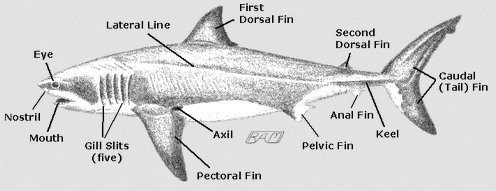
\includegraphics{Images/sharkimg.png}    
    \caption[This is another figure.] {This is another figure as an example. Please note that the Editorial Office does not allow borders around figures. Used with permission from Martin, R. Aidan.  2003. }
    \label{fig:my_label}
\end{figure}{}
\section{Placement Specifiers}

Floats are used to allow LaTeX to handle figures while maintaining the best possible presentation. However, there may be times when you disagree, and a typical example is with its positioning of figures. 
The placement specifier parameter exists as a compromise, and its purpose is to give the author a greater degree of control over where certain floats are placed. As you can see in Figure \ref{fig:my_label}A this is a shark. As you can see in \ref{tbl1} this is a something.

\begin{table}[H]
\caption{Specifier Table}
\begin{tabular}{l p{14cm} }
\hline
Specifier & Permission \\ \hline
h & Place the float here, i.e., approximately at the same point it occurs in the source text (however, not exactly at the spot) \\
\\
t & Position at the top of the page.  \\
\\
b & Position at the bottom of the page.  \\
\\
p & Put on a special page for floats only.  \\
\\
! & Override internal parameters LaTeX uses for determining "good" float positions. \\
\\
H & Places the float at precisely the location in the LaTeX code. \\
\hline
\end{tabular}
\end{table}

\newpage

%An example of a specifier parameter is shown below to force a figure into place where it is mentioned in text: 
%\begin{verbatim}
%\begin{figure}[h!]
%    \begin{center}
 %       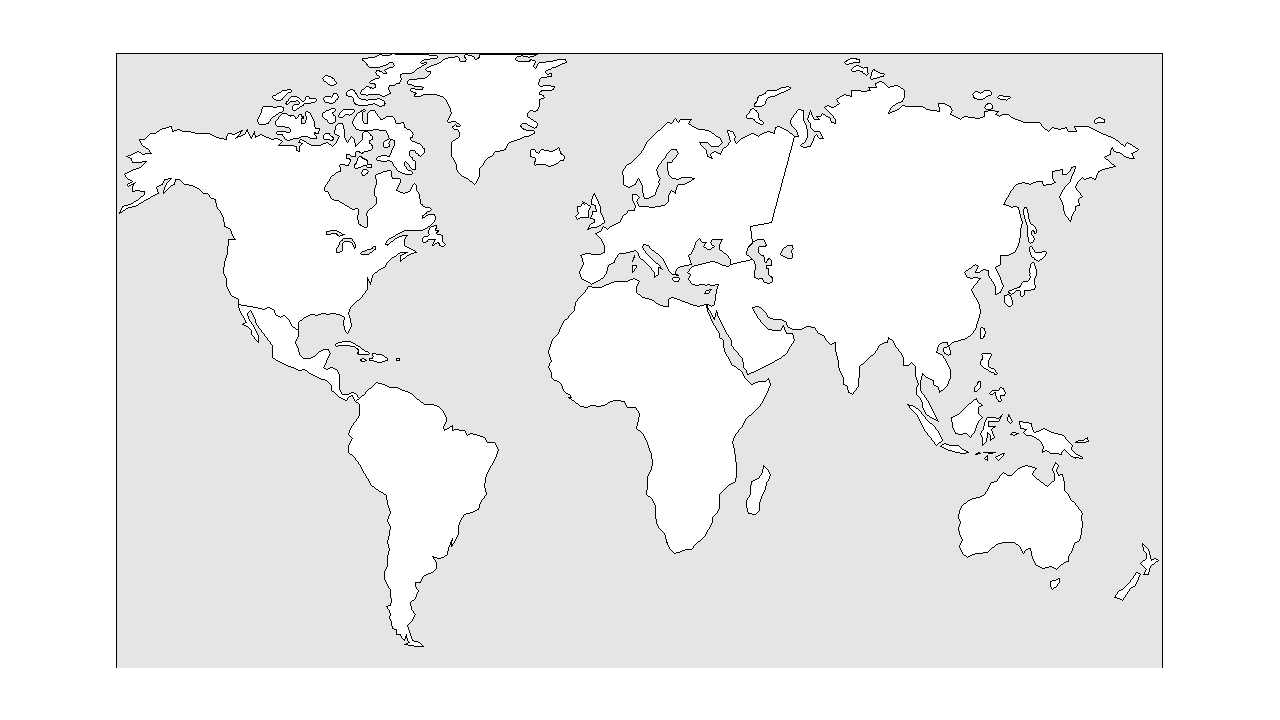
\includegraphics[width=0.9\textwidth]{./theworld.png}
%    \end{center}
%     \caption[My short caption.]{My full caption in curly brackets.}
%\end{figure}
%\end{verbatim}

